\chapter{Généralité sur le développement web }
\section{Introduction }
\par Depuis l'avènement des réseaux informatiques, l’Internet qui est un réseau
informatique global ne cesse de se développer, et quand on dit Internet on
pense web et application web.
\par Une application web est généralement composée de deux parties différentes,
le Front-end qui représente tout ce qui est visible par l’utilisateur du web,
et le Back-end qui forme la logique et le comportement de l’application web.
\par Dans ce chapitre nous allons parler des différents aspects autour des
technologies web que nous allons utiliser durant le développement de notre
application.

\section{Réseaux informatique}
\par Un réseau informatique peut être décrit comme étant un ensemble
d'appareils électroniques qui échangent des informations entre eux. L’internet
conçu dans les années soixante est une série d'énorme de réseaux informatique
qui permettent à de nombreux ordinateurs de se connecter et de communiquer
entre eux à l'échelle mondial.\cite{ref6}
\subsection{Web }
\par Le world wide web (WWW) communément appelé le web, créé dans les années
quatre-vingt, est un système d'information mondial basé sur Internet. Le Web
est un système de documents hypertextes interconnectés contenus sur Internet,
et qui permet d’échanger des information sur Internet en communiquant via le
protocol HTTP.\cite{ref6}
\subsection{Protocol HTTP et HTTPs }
\par L’Hypertext Transfer Protocol, généralement abrégé HTTP. HTTP est un
protocole de communication client-serveur, il est la base de tout échange de
données sur le web. HTTP est un protocole de la couche application conçu pour
transférer des informations entre des appareils connectés en réseau.
\par HTTPS ou HyperText Transfer Protocol Secure est une version plus avancée
et sécurisée de l’HTTP, ce qui signifie que les données échangées entre le
client et le serveur sont chiffrées et ne peuvent en aucun cas être espionnées
ou modifiées.
\par HTTP fonctionne comme un protocole de requête-réponse entre un client et
un serveur, et pour cela HTTP dispose de plusieurs méthode, et les plus
utiliser d’entre elle sont GET, POST, PUT, DELETE.
\begin{itemize}[label=\textbullet] 
\item \textbf{GET}: est utilisée pour lire (ou récupérer) une représentation
d'une ressource.
\item \textbf{POST}: est le plus souvent utilisé pour créer une nouvelle
ressource.
\item \textbf{PUT}: est utilisé pour modifier (mettre à jour) une donnée.
\item \textbf{DELETE}: est utilisé pour supprimer une donnée.
\end{itemize}
\subsection{Architecture Client-Serveur }
\par Les applications web fonctionnent selon l'architecture client/serveur, qui
représente l’environnement dans lequel des applications de machines type
clientes communiquent avec des applications de machines de type
serveurs.\cite{ref6}
\begin{itemize}[label=\textbullet]
\item \textbf{Client}: est celui qui demande un ou des services.
\item \textbf{Serveur}: est celui qui fournit les services demandés.
\end{itemize}
\subsection{Architecture RestAPI }
\par REST ou REpresentational State Transfer est un style architectural qui
définit un ensemble de contraintes à utiliser pour créer des services Web.
L'API (Application Program Interface) REST est un moyen d'accéder aux services
Web de manière simple et flexible sans aucun traitement.
\par REST fonctionne au-dessus du protocole HTTP. Il tire parti des capacités
natives de HTTP, telles que GET, PUT, POST et DELETE. Lorsqu'une requête est
envoyée à une API RESTful, la réponse (la "représentation" de la "ressource"
d'information recherchée) est renvoyée sous format JSON, XML ou HTML. Une API
RESTful est définie par une adresse Web, ou URI (Uniform Resource Identifier),
qui suit généralement une convention de dénomination.\cite{ref7}
\begin{figure}[H]
\centering
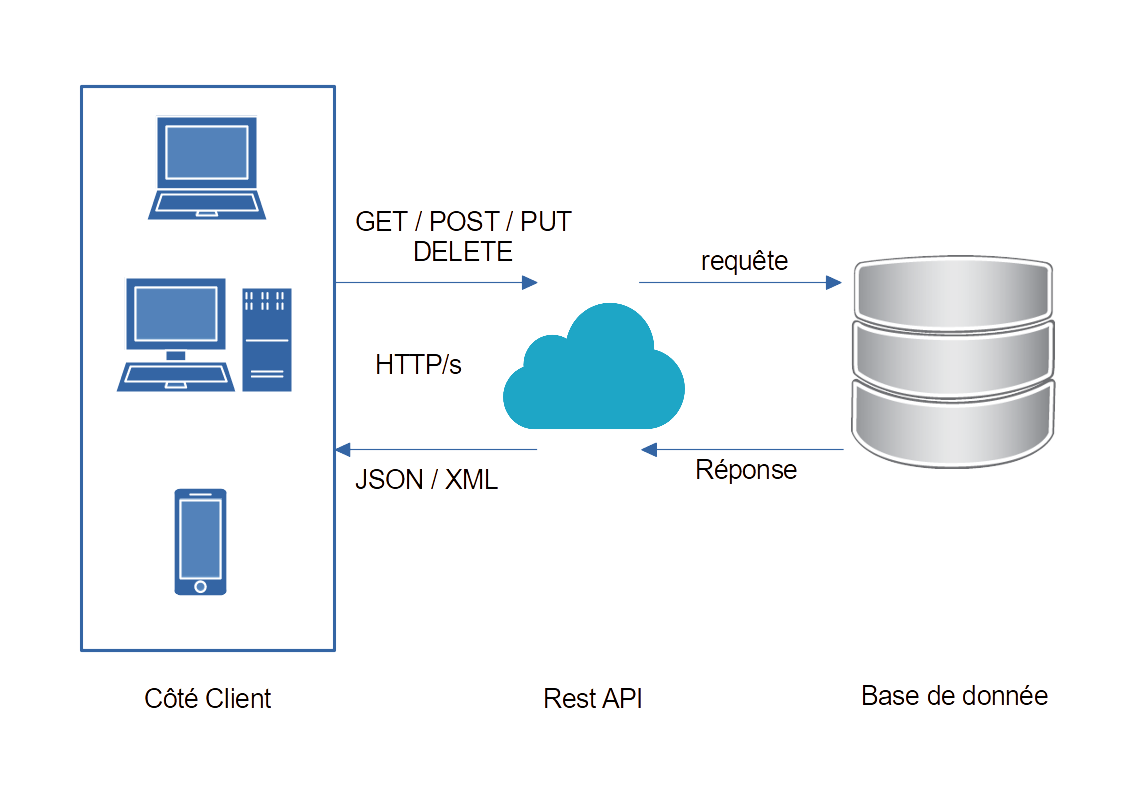
\includegraphics[scale=0.4]{Figures/figure arch restapi.png}
\caption{Architecture Rest API}.
\label{fig:my_label}
\end{figure}
\section{Développement web }
\par Ou développement de site web, est le travail impliqué dans la création, la
construction et à la maintenance de sites web et d’applications web hébergé sur
intranet ou Internet . Mais cela peut inclure aussi la conception, la
publication, la programmation et la gestion de base de données.
\subsection{Application web  }
\par Une application web est une interface web applicative disponible
uniquement sur le web et accessible via un navigateur internet. C’est une
application qui peut être hébergée en cloud ou sur des serveurs dédiés. Toutes
les données sont stockées sur un serveur web.\cite{ref8}
\par Une application web se compose de deux parties comme on a précisé en haut,
une partie front-end et une partie back-end.
\subsubsection{Back-end }
\par Back-end c’est la notation qui englobe tout ce qui s'exécute en côté
serveur, le serveur (hardware)  qui est un ordinateur qui exécute un système
d’exploitation tel que Windows et Ubuntu, et permet de déployer un serveur
(software) qui expose un port ou plusieur port sur Internet, grâce à un URL
(Uniform Resource Locator), les fichiers tel que les fichiers HTML et autres
tel que des fichier JavaScript, CSS, Images, vidéo, audio..etc exposée par le
serveur et sont accessible par le côté front-end (client).
\par D'autre part, le backend se compose généralement de trois parties : un
serveur, une application et une base de données \cite{ref9}, parfois la partie
serveur et application se fusionne en une partie, et c’est l'avantage
d’utiliser quelque technologie et langage tel que NodeJs (le fameux framework
ExpressJs), et dans d’autre cas le serveur et l’application sont séparés, c’est
le cas pour l’utilisation du langage PHP qui exige d’avoire un serveur comme
Apache à part qui permet d'exécuter les script PHP et les renvoyer le résultat
de la requête au client. Et dans les deux cas l’application a besoin de stocker
les information qui peut être représenté sous différents format (texte, images,
binaire…), et pour cela on utilise des base de données et des SGBD (systèmes de
gestion de base de données) tel que Mysql, MariaDB..etc.
\subsubsection{Front-end }
\par Dans le contexte Web, le front-end est la partie que l'utilisateur voit et
interagit avec. Concevoir et développer une telle interface web frontale,
certains outils et technologies doivent être utilisées, qui sont généralement
une combinaison de HTML, CSS et JavaScript étant tous contrôlés par le
navigateur.\cite{ref9}
\par Il existe plusieurs navigateurs Web qui permettent de surfer sur le net
comme Google Chrome et Mozilla FireFox, tous les navigateurs existants sont
basés sur les trois technologies suivantes : HTML, CSS, JavaScript.
\par HTML (Hypertext Markup Language), comme définie dans le dictionnaire
Larousse, est un langage de description de documents servant à présenter des
pages Web et à préciser à l'aide de balises les liens hypertextes avec d'autres
documents. HTML représente la squelette de la page web contenant le contenu
sous format texte. d’autre part CSS (Cascading Style Sheets) ou feuilles de
style en cascade, qui est utilisé pour décrire la présentation d’un document
HTML ou XML, autrement dit CSS décrit comment les éléments doivent être chargés
par rapport à l'écran (la couleur, la taill…etc).\cite{ref10}
\par D'après le dictionnaire Larousse, Javascript est un langage de
programmation utilisé pour écrire des appelettes incorporables à des documents
au format HTML. En gros, Javascript décrit le comportement de la page web.